\PassOptionsToPackage{sols}{handout}
\documentclass[main]{subfiles}
\setcounterrefbeforedot{chapter}{m-ws5-4}
\setcounterrefafterdot{section}{m-ws5-4}
\addtocounter{section}{-1}
\usepackage{solutions}

\begin{document}

\ifSubfilesClassLoaded{%
  \chaptermark{\chapterfive}
}{}

\section{Properties of the Definite Integral} \label{ws5-4}

\begin{problemonly}
    \begin{framed}

\textbf{Key Ideas}:

\begin{itemize}[topsep=0pt,partopsep=0pt,parsep=8pt,itemsep=0pt]

\item You should know the basic properties of the definite integral
  (listed on pg. 738) and be able to use them to simplify expressions
  involving definite integrals. 

\item You should understand the definition of the ``area function'' $A(x)=\displaystyle \int_a^x f(t)\,dt$
and be able to interpret it in terms of signed area and (if $f$ is
  a rate function) net change. The capital $A$ represents ``Area'' and 
  for ``Accumulation'' and for ``net change in Amount'' when $f$ is
  a rate function.

\item If $f$ is a function whose graph is made up of simple geometric
  shapes, you should be able to find a formula for the area function $A(x)$.

\item You should understand why two area functions $A(x)=\displaystyle \int_a^x f(t)\,dt$ and 
  $B(x)=\displaystyle \int_b^x f(t)\,dt$ for the same function $f$ with different anchors 
  differ by a constant and be able to find that constant.

\end{itemize}
\end{framed}
\end{problemonly}

\begin{enumerate}
\item 
  \begin{problem}[\vfill]
    Remember that we have 3 main ways of thinking about the definite
    integral.  What are they?
  \end{problem}

  \begin{solution}
    \begin{enumerate}[topsep=0pt,label=\arabic*.]
      \item If $a < b$, we visualize $\displaystyle \int_a^b f(x)\,dx$
        as the signed area under $f$ from $a$ to $b$.
      \item If $f$ is a rate function, then we interpret $\displaystyle
        \int_a^b f(x)\,dx$ as the net change in amount from $x = a$ to
        $x = b$.  For instance, if $f(x)$ represents the rate at which
        water is entering or leaving a pool at time $x$, then
        $\displaystyle \int_a^b f(x)\,dx$ is the net change in amount of
        water from time $a$ to time $b$, or (amount of water at time
        $b$) $-$ (amount of water at time $a$).
      \item $\displaystyle \int_a^b f(x)\,dx$ is defined to be
        $\displaystyle \lim_{n \to \infty} R_n$ or $\displaystyle
        \lim_{n \to \infty} L_n$.
      \end{enumerate}
  \end{solution}

  \textbf{Reminder!} These are not mutually exclusive interpretations! We want to be comfortable with and understand all three, and then be able to appeal to the interpretation that a given problem calls for. 

\item 
  \emph{Properties of the Definite Integral.}

  \begin{enumerate}[topsep=0pt]

  \item
    \note{This property can be a confusing one for students, since we've
      only ever really thought about $\displaystyle \int_a^b f(t)\,dt$ as
      representing signed area / net change when $a < b$.  The net change
      interpretation is convincing here, but I will say a little bit about
      how this really comes from our \emph{definition} of the definite
      integral as a limit of Riemann sums ($\Delta t$ will be negative,
      etc.).

      We'll generalize this to $\displaystyle \int_b^a f(t)\,dt = -
      \int_a^b f(t)\,dt$.}

    \begin{problem}
    
    \begin{enumerate}[topsep=0pt]
      \item How do $\displaystyle \int_1^4 f(t)\,dt$ and 
      $\displaystyle \int_4^1 f(t)\,dt$ relate? 
      \pspace{\stretch{0.5}}
      
      \item Generalize this result.
      \pspace{\nstretch{0.5}}
    \end{enumerate}
    \end{problem}

    \begin{solution}
      They are negatives of each other; that is, $\boxed{\int_4^1
      f(t)\,dt\, = - \int_1^4 f(t)\,dt.}$
      
      This makes sense if you think
      about the net change interpretation: if $f(t)$ is the rate of change
      of the amount of water in a pool at time $t$, then
      \[ \int_1^4 f(t)\,dt = (\text{amount of water in pool at
        time $4$}) - (\text{amount of water in pool at time $1$}),\] while
      \[\displaystyle \int_4^1 f(t)\,dt = (\text{amount of water in pool at
        time $1$}) - (\text{amount of water in pool at time $4$}).\]

      This idea generalizes: $\boxed{\int_b^a f(t)\,dt\, = - \int_a^b
      f(t)\,dt}$ for any $a$ and $b$.
    \end{solution}

  \item

    \note{This first statement should be quite clear from pictures, and 
    then we'll
      generalize as $\displaystyle \int_a^b f(t)\,dt + \int_b^c f(t)\,dt\, =
      \int_a^c f(t)\,dt$. That will be more challenging. I plan to draw
      an interval
      \begin{center}
        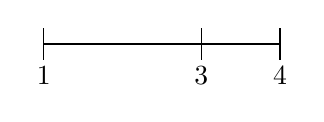
\begin{tikzpicture}
            \draw (1,0.2) -- (1,-0.2);
            \draw (3,0.2) -- (3,-0.2);
            \draw (4,0.2) -- (4,-0.2);
            \draw (1,0) -- (4,0);
            \path (1,-0.4) node {$1$} (3,-0.4) node {$3$}
              (4,-0.4) node {$4$};
        \end{tikzpicture}
      \end{center}
      and have everyone work through these. Then I'll have each group
      work through one of the other 4 permutations. I will draw the
      following picture
      \begin{center}
        \begin{tikzpicture}[
            declare function={
            f(\x) = (\x<2)*(+-0.25*\x^3+0.75*\x^2+1.0963e-61*\x^1+0.5*\x^0) +
                and(\x>=2,\x<3)*(+0.5*\x^3+-3.75*\x^2+9*\x^1+-5.5*\x^0) +
                and(\x>=3,\x<=4)*(+-0.25*\x^3+3*\x^2+-11.25*\x^1+14.75*\x^0);
                }
            ]
          \begin{axis}[xmin=0.5,xmax=4.5,ymin=0,
            hide y axis, xtick={1,3,4},axis equal image]
            \addplot[domain=1:4]{f(x)};
            \draw[dashed] (1,1) -- (1,0);
            \draw[dashed] (3,1.25) -- (3,0);
            \draw[dashed] (4,1.75) -- (4,0);
            \node at (2,0.75) {\Large $A$};
            \node at (3.5,0.75) {\Large $B$};
          \end{axis}
        \end{tikzpicture}
      \end{center}
      and students can interpret the definite integrals in terms of $\pm A$
      and $\pm B$. This exercise will allow students to practice the
      endpoint reversal property.}
      
    \begin{enumerate}[topsep=0pt]

    \item
    \begin{problem}[\stretch{0.5}]
      Can you simplify $\displaystyle \int_1^3 f(t)\,dt\, + \int_3^4
      f(t)\,dt$?
    \end{problem}

    \begin{solution}
      Let  $A=\displaystyle \int_1^3 f(t)\,dt$ and let 
      $\displaystyle B=\int_3^4 f(t)\,dt$.
      \begin{center}
        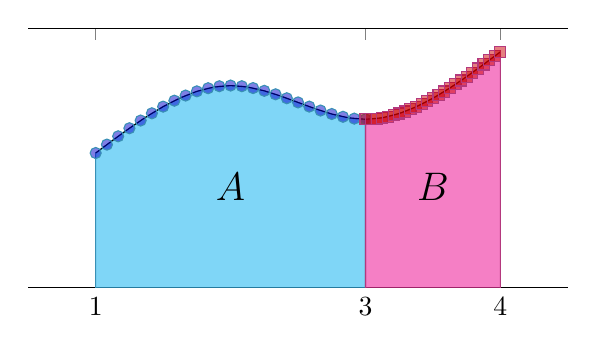
\begin{tikzpicture}[
            declare function={
            f(\x) = (\x<2)*(+-0.25*\x^3+0.75*\x^2+1.0963e-61*\x^1+0.5*\x^0) +
                and(\x>=2,\x<3)*(+0.5*\x^3+-3.75*\x^2+9*\x^1+-5.5*\x^0) +
                and(\x>=3,\x<=4)*(+-0.25*\x^3+3*\x^2+-11.25*\x^1+14.75*\x^0);
                }
            ]
          \begin{axis}[xmin=0.5,xmax=4.5,ymin=0,
            hide y axis, xtick={1,3,4},axis equal image]
            \addplot+[domain=1:3, fill=cyan, fill opacity=0.5,
            draw=cyan!70!black] {f(x)} \closedcycle; %
            \addplot+[domain=3:4, fill=magenta, fill opacity=0.5,
            draw=magenta!70!black] {f(x)} \closedcycle; %
            \addplot[black,domain=1:4] {f(x)}; %
            \draw (2,0.75) node[black] {\Large $A$}; %
            \draw (3.5,0.75) node[black]
            {\Large $B$}; %
          \end{axis}        
        \end{tikzpicture}
      \end{center}
      From this picture, we can see that $\boxed{\int_1^3 f(t)\,dt\,
      + \int_3^4 f(t)\,dt\, = \int_1^4 f(t)\,dt.}$

      This makes sense from a net change perspective, as the sum of the
      net change from $t=1$ to $t=3$ and the net change from $t=3$ to $t=4$
      is equal to the net change from $t=1$ to $t=4$.
    \end{solution}

    \item 
    \begin{problem}[\stretch{0.5}]
        Does 
        $\displaystyle \int_1^4 f(t)\,dt\, + \int_4^3 f(t)\,dt\, 
        = \int_1^3 f(t)\,dt$?
    \end{problem}

    \begin{solution}
        We know that $\displaystyle \int_1^4 f(t)\,dt\, 
            = \int_1^3 f(t)\,dt\, + \int_3^4 f(t)\,dt\, = A+B$.
            
            Based on part (a),
            $\displaystyle \int_4^3 f(t)\,dt = -\int_3^4 f(t)\,dt = -B$.

            Thus, $\displaystyle \int_1^4 f(t)\,dt\, 
            + \int_4^3 f(t)\,dt\, = (A+B) - B = A = \boxed{\int_1^3 f(t)\,dt}$.

            In terms of net change, this is saying that the net change from $t=1$
            to $t=4$ plus the net change \ul{from $t=4$ to $t=3$} is equal to the
            net change from $t=1$ to $t=3$.
    \end{solution}

    \item
    \begin{problem}
        Does $\displaystyle \int_a^b f(t)\,dt\, + \int_b^c f(t)\,dt\,
        = \int_a^c f(t)\,dt$ even if $b$ is not between $a$ and $c$? Try these.
    \end{problem}
   \begin{multicols}{2}
        \begin{enumerate}
            \item $\displaystyle \int_3^4 f(t)\,dt\, 
            + \int_4^1 f(t)\,dt\,
            \overset{?}{=} \int_3^1 f(t)\,dt$
            \item $\displaystyle \int_4^1 f(t)\,dt\, + \int_1^3 f(t)\,dt\,
            \overset{?}{=} \int_4^3 f(t)\,dt$
            \item $\displaystyle \int_3^1 f(t)\,dt\, + \int_1^4 f(t)\,dt\,
            \overset{?}{=} \int_3^4 f(t)\,dt$ 
            \item $\displaystyle \int_4^3 f(t)\,dt\, + \int_3^1 f(t)\,dt\,
            \overset{?}{=} \int_4^1 f(t)\,dt$
        \end{enumerate}
        \end{multicols}
        \bigskip
        \bigskip
        \begin{solution} 
        \fbox{These are all true.} We can use part (a) to rewrite them as 
        \begin{enumerate}
            \item $\displaystyle \int_3^4 f(t)\,dt\, 
            - \int_1^4 f(t)\,dt\,
            = - \int_1^3 f(t)\,dt$
            \item $\displaystyle - \int_1^4 f(t)\,dt\, + \int_1^3 f(t)\,dt\,
            = - \int_3^4 f(t)\,dt$
            \item $\displaystyle -\int_1^3 f(t)\,dt\, + \int_1^4 f(t)\,dt\,
            = \int_3^4 f(t)\,dt$ 
            \item $\displaystyle -\int_3^4 f(t)\,dt\, - \int_1^3 f(t)\,dt\,
            = - \int_1^4 f(t)\,dt$
        \end{enumerate}
        These are all rearrangements of
        $\displaystyle \int_1^3 f(t)\,dt\,
      + \int_3^4 f(t)\,dt\, = \int_1^4 f(t)\,dt$.
        \end{solution}
    \end{enumerate}

    \pspace{\vfill}
  \item

    \note{This should be clear from both a signed area and net change
      perspective.  (If Anna and Bob are running a race and Anna is always
      3 times as fast as Bob, then she'll go 3 times as far.)  We'll
      generalize to $\displaystyle \int_a^b k f(t)\,dt = k \int_a^b
      f(t)\,dt$.}

    \begin{problem}
    \begin{enumerate}
        \item 
        How does $\displaystyle \int_a^b 3 f(t)\,dt$ relate to
        $\displaystyle \int_a^b f(t)\,dt$?  Why? Can you argue both from
         a signed area perspective and a net change perspective?
         \pspace{\stretch{1}}

         \item
          Generalize.
          \pspace{\nstretch{0.5}}
    \end{enumerate}
    \end{problem}

    \begin{solution}
      $\boxed{ \int_a^b 3 f(t)\,dt = 3 \int_a^b f(t)\,dt}$.  
      In terms of signed area: the
      graph of $3 f(t)$ is just the graph of $f(t)$ stretched vertically
      by a factor of 3 (to be 3 times as tall), so the area under $3 f(t)$
      from $t = a$ to $t = b$ is 3 times the area under $f(t)$ from $t =
      a$ to $t = b$. In terms of net change: the change in amount
      when the rate of change is $3f(t)$ will be 3 times the change in
      amount when the rate is $f(t)$.  

      In general, 
      $\boxed{\displaystyle \int_a^b kf(t)\,dt = k\int_a^b f(t)\,dt}$.
    \end{solution}

  \item

    \note{Here, it may help to use the net change interpretation; for
      example, if a swimming pool is being filled by two pipes, the net
      change in water is the amount of water added by the first pipe plus
      the amount of water added by the second pipe.}

    \begin{problem}[\vfill]
      How does $\displaystyle \int_a^b \left[f(t) + g(t)\right]\,dt\,$
      relate to
      $\displaystyle \int_a^b f(t)\,dt$ and $\displaystyle \int_a^b
      g(t)\,dt$?  Why?
    \end{problem}

    \begin{solution}
      $\boxed{\int_a^b \left[f(t) + g(t)\right]\,dt\, 
      = \int_a^b f(t)\,dt\, +
      \int_a^b g(t)\,dt}$.  One way to understand this is by thinking about
      net change.  For example, imagine that a swimming pool is being
      filled by two pipes, one filling at the rate $f(t)$ and the other at
      the rate $g(t)$.  Then, the total rate at which water is being added
      to the pool at time $x$ is $f(t) + g(t)$, and
      \[ 
      \underbrace{\left(
            \begin{tabular}{c}
              \text{amount of water} \\
              \text{added between} \\
              \text{time $a$ and time $b$}
            \end{tabular} \right)}_{\displaystyle 
            \int_a^b \left[ f(t) + g(t)\right]\,dt} =
        \underbrace{\left( 
            \begin{tabular}{c}
              \text{amount of water added} \\
              \text{by pipe 1 between} \\
              \text{time $a$ and time $b$}
            \end{tabular} \right)}_{\displaystyle \int_a^b f(t)\,dt} +
        \underbrace{\left( 
            \begin{tabular}{c}
              \text{amount of water added} \\
              \text{by pipe 2 between} \\
              \text{time $a$ and time $b$}
            \end{tabular} \right)}_{\displaystyle \int_a^b g(t)\,dt}
        \]
    \end{solution}

    \item

    \note{
    You might also draw two functions such that their product is zero to
    illustrate a counterexample.
    \begin{center}
        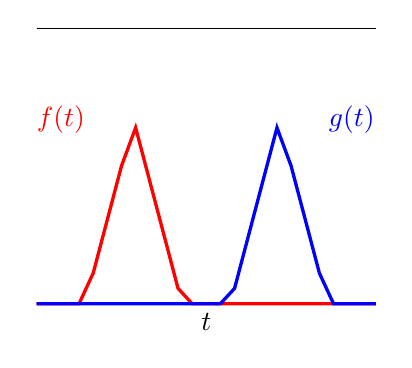
\begin{tikzpicture}[declare function ={
        f(\x) = and(\x>=-1,\x<0)*(1+\x)+and(\x>=0,\x<=1)*(1-\x);
        }]
            \begin{axis}[
            xmin = -2, xmax = 5,
            ymin = 0, ymax = 1.5,
            xlabel=$t$,
            xtick=\empty, hide y axis,
            height = 2in,
            clip = false,
            ]
            \addplot[very thick,red,domain=-2:5] {f(x)};
            \node[red] at (-1.5,1) {$f(t)$};
            \addplot[very thick,blue,domain=-2:5] {f(x-3)};
            \node [blue] at (4.5,1) {$g(t)$};
            \end{axis}
        \end{tikzpicture}
    \end{center}
    The incorrect equation is also dimensionally inconsistent 
    (units don't match.)
    }
    
    \begin{problem}[\vfill]
        Caution: $\displaystyle \int_a^b f(t)g(t)\,dt\, \neq
        \int_a^b f(t)\,dt\, \int_a^b g(t)\,dt$. 
        
        Show that this does not work
        for $\displaystyle \int_0^2 f(t)g(t)\,dt$ if $f(t)=2$ and $g(t)=1$.
    \end{problem}

    \begin{solution}
        If $f(t)=2$ and $g(t)=1$, then 
        $\displaystyle\int_0^2 f(t)g(t)\,dt\, = \int_0^2 2\,dt\,=4$.
        
        However, 
        $\displaystyle\int_0^2 f(t)\,dt\, \int_0^2 g(t)\,dt\, =
        \int_0^2 2\,dt\, \int_0^2 1\,dt = 4\cdot 2 = 8$.
    \end{solution}

  \end{enumerate}

\end{enumerate}

\begin{framed}
  \textbf{Summary.}
  \begin{enumerate}[topsep=0pt,label=\arabic*.]
  \item Endpoint Reversal Property

    $\displaystyle \int_b^a f(t)\,dt\, = \solonly{\boxed{-\int_a^b f(t)\,dt}}$

  \item Splitting Interval Property
  
    $\displaystyle \int_a^b f(t)\,dt\, + \int_b^c f(t)\,dt\, = \solonly{\boxed{
        \int_a^c f(t)\,dt }}$

  \item Constant Multiple Property
  
    If $k$ is a constant, $\displaystyle \int_a^b k f(t)\,dt\, =
    \solonly{\boxed{k \int_a^b f(t)\,dt}}$

  \item Additive Integrand Property
  
    $\displaystyle \int_a^b \left[f(t) + g(t)\right]\,dt\, 
    = \solonly{\boxed{\int_a^b
        f(t)\,dx +\int_a^b g(t)\,dx}}$
  \end{enumerate}
\end{framed}

\pspace{\newpage}

\begin{enumerate}[resume]
\item 
  \note{This is just practice applying the properties.}

  Suppose you know that $\displaystyle \int_2^5 f(t)\,dt = 7$.  Do you have
  enough information to evaluate each of the following integrals?  If so,
  evaluate; if not, explain why not.
  \begin{enumerate}
  \item
    \begin{problem}[\vfill]
      $\displaystyle \int_2^5 [f(t) + 4]\,dt$
    \end{problem}

    \begin{solution}
      Yes; we can rewrite this as
      \begin{align*}
        \int_2^5 [f(t) + 4]\,dt &= \int_2^5 f(t)\,dt + \int_2^5 4\,dt
        \text{ by Property
            {{4.}}} \\
        &= 7 + \int_2^5 4\,dt \\
        &= 7 + 12 \text{ by interpreting $\displaystyle \int_2^5 4\,dt$ as
          a signed area} \\
        &= \boxed{19}
      \end{align*}
    \end{solution}

  \item

    \note{Here, I'll probably try to get them to see (from a picture) that
      they \emph{can} evaluate $\displaystyle \int_{-2}^1 f(t + 4)\,dt$.}

    \begin{problem}[\vfill]
      $\displaystyle \int_2^5 f(t + 4)\,dt$
    \end{problem}

    \begin{solution}
      There is not enough information.  The graph of $f(t + 4)$ is the
      graph of $f(t)$ shifted left by $4$ units, so the behavior of $f(t
      + 4)$ on $[2, 5]$ has nothing to do with the behavior of $f(t)$ on
      $[2, 5]$. 
    \end{solution}

  \item
    \begin{problem}[\vfill]
      $\displaystyle \int_5^2 4 f(t)\,dt$
    \end{problem}

    \begin{solution}
      Yes; we can rewrite this as
      \begin{align*}
        \int_5^2 4 f(t)\,dt &= - \int_2^5 4 f(t)\,dt \text{
            by the Endpoint Reversal Property} \\
        &= - 4 \int_2^5 f(t)\,dt \text{ by the Constant Multiple Property} \\
        &= -4 \cdot 7 \\
        &= \boxed{-28}
      \end{align*}
    \end{solution}

  \item
    \begin{problem}[\vfill\newpage]
      $\displaystyle \int_2^4 [f(t) + t]\,dt + \int_4^5 f(t)\,dt$
    \end{problem}

    \begin{solution}
      Yes; we can rewrite this as
      \begin{align*}
        \int_2^4 [f(t) + t]\,dt + \int_4^5 f(t)\,dt &= \int_2^4 f(t)\,dt +
        \int_2^4 t\,dt + \int_4^5 f(t)\,dt \text{ by 
        the Additive Integrand Property} \\
        &= \int_2^5 f(t)\,dt + \int_2^4 t\,dt \text{ by the Splitting Interval
        Property} \\
        &= 7 + \int_2^4 t\,dt \\
        &= 7 + 6 \text{ by visualizing $\displaystyle \int_2^4 t\,dt$ as a
          signed area} \\
        &= \boxed{13}
      \end{align*}
    \end{solution}

  \end{enumerate}

\item 
  \note{This problem is motivation for introducing the area function 
  $A(x)$.} 

  At the Blue Bell ice cream factory, milk is stored in a 40,000 gallon
  tank.  Let $f(t)$ be the rate (in gallons per hour) of milk flowing into
  and out of the tank on a certain day at time $t$, 
  where $t$ is measured in hours
  after noon.  At noon, there are 15,000 gallons of milk in the tank.
  \begin{enumerate}
  \item
    \begin{problem}[\vfill]
      How much milk is in the tank at 7 pm?  Your answer should involve a
      definite integral.
    \end{problem}

    \begin{solution}
      $\displaystyle 15,000 + \int_0^7 f(t)\,dt$. 
    \end{solution}

  \item
    \note{After we do this, I'll point out that it's quite natural to want
      to think of this as a function of $x$ and introduce the notation
      $A(x) = \displaystyle \int_3^x f(t)\,dt$. It's nice to point
      out that this integral can be thought of as an area function or
      as an accumulation of amount when $f$ is a rate function.}

    \begin{problem}[\vfill]
      How much milk is in the tank $x$ hours after noon?
    \end{problem}

    \begin{solution}
      $\displaystyle 15,000 + \int_0^x f(t)\,dt$. 
    \end{solution}

  \item
    \begin{problem}[\vfill]
        Let $A(x) = \displaystyle\int_0^x f(t) \, dt$.  What does $A(7)$ represent?
    \end{problem}

    \begin{solution}
      This means $\displaystyle \int_0^7 f(t)\,dt$, which represents
      the net change in the amount of milk from $t=0$ to $t=7$, or
      (amount of milk in the tank at 7 pm) $-$ (amount of milk in the tank
      at noon).
    \end{solution}

  \item
    \begin{problem}[\vfill]
      What does $A(x)$ represent?
    \end{problem}

    \begin{solution}
      This is $\displaystyle \int_0^x f(t)\,dt$, which is the
      net change in the amount of milk from $t=0$ to $t=x$, or
      (amount of milk in the tank $x$ hours after noon) $-$ (amount of
      milk in the tank at noon).
    \end{solution}

  \item

    \note{This is basically Part 1 of the Fundamental Theorem of Calculus,
      which we'll talk about more next time.}

    \begin{problem}[\vfill\newpage]
      Let $M(x)$ be the amount of milk in the tank $x$ hours after noon.
      How would you express ``the instantaneous rate at which milk is
      flowing into/out of the tank at 6 pm'' in terms of $M(x)$?  In terms of
      $f$?  In terms of $A(x)$?
    \end{problem}

    \begin{solution}
      The instantaneous rate at which milk is flowing into/out of the tank
      at 6 pm is $M'(6)$ or $f(6)$.

      Let's figure out how to express this in terms of $A$.  From
      {{{{\#4}}(b)}}, $M(x) = 15,000 + A(x)$.
      Differentiating this, $M'(x) =A'(x)$, so $M'(6) = A'(6)$.

      Therefore, we can express ``the instantaneous rate at which milk is
      flowing into/out of the tank at 6 pm'' as $\boxed{M'(6) =
        A'(6) = f(6)}$.
    \end{solution}

  \end{enumerate}

\item 
  \note{This problem is meant to familiarize students with the notation we
    use for the area function.  If there is time to get it all up on the
    board, then we'll also look at the values to see that $A(x)$ and
    $B(x)$ differ by a constant and that we can ``explain''that
    constant as $\displaystyle \int_0^2 f(t)\,dt$.  If there is still time
    after that, I'll have them try to sketch $A(x)$ and $B(x)$.
    \#5 on the PSET is very very similar.}

  Here is the graph of a function $f$.  (The graph is composed of two
  straight line segments and one semicircle of radius 3.)  

  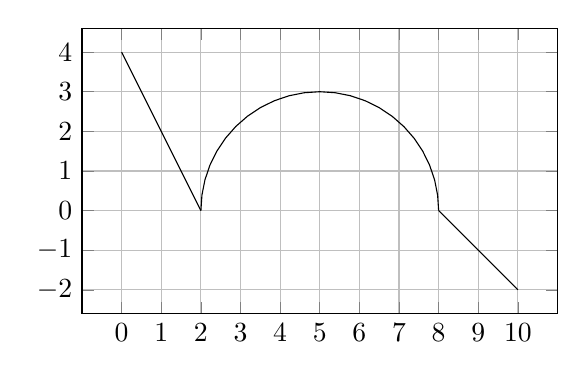
\begin{tikzpicture}
    \begin{axis}[xtick={0, 1, ..., 10}, ytick={-2, -1, ..., 4},
      grid=major, cycle list=black, axis equal=true, ymin=-2, ymax=4,
      clip=false, width=3in, height=2.05in, axis line style={shorten >=-8pt}]
      \addplot+[sharp plot] coordinates { (0, 4) (2, 0) };
      \addplot+[domain=0:180] ({3*cos(x) + 5}, {3*sin(x)}); 
      \addplot+[sharp plot] coordinates { (8, 0) (10, -2) };
    \end{axis}
  \end{tikzpicture}

  Let $A(x) = \displaystyle \int_0^x f(t)dt$ and let
  $B(x) = \displaystyle \int_2^x f(t)dt$. 
  Evaluate each of the following.

  \begin{center}
    \renewcommand{\arraystretch}{3}
    \begin{tabular}{>{$\displaystyle}l<{$} | >{$\displaystyle}l<{$}}
      \hline
      A(0) = \solonly{\boxed{\int_0^0 f(x)\,dx = 0}}
      \probonly{\text{\hspace{1in}}} & 
      B(0) = \solonly{\boxed{\int_2^0 f(x)\,dx = 
      - \int_0^2 f(x)\,dx =
          -4}} \probonly{\text{\hspace{1in}}} \\  
      \hline
      A(2) = \solonly{\boxed{\int_0^2 f(x)\,dx = 4}}  &
      B(2) = \solonly{\boxed{\int_2^2 f(x)\,dx = 0}}  \\ \hline
      A(5) = \solonly{\boxed{\int_0^5 f(x)\,dx = 4+\frac{9}{4}\pi}}  &
      B(5) = \solonly{\boxed{\int_2^5 f(x)\,dx = \frac{9}{4}\pi}}  \\ 
      \hline
      A(8) = \solonly{\boxed{\int_0^8 f(x)\,dx = 4+\frac{9}{2}\pi}}  &
      B(8) = \solonly{\boxed{\int_2^8 f(x)\,dx = \frac{9}{2}\pi}}  \\ 
      \hline
      A(10) = \solonly{\boxed{\int_0^{10} f(x)\,dx = 2+\frac{9}{2}\pi}}
      &
      B(10) = \solonly{\boxed{\int_2^{10} f(x)\,dx 
      = \frac{9}{2}\pi-2}}
      \\
      \hline
    \end{tabular}    
    \renewcommand{\arraystretch}{1}
  \end{center}

  \begin{problem}[3in]
    Do you see any relationship between $A(x)$ and $B(x)$?  Can
    you explain this relationship?
    
\bigskip

    When $f$ is positive, what can you say about $A(x)$?

\bigskip
     Can the same be said about $B(x)$?
  \end{problem}

  \begin{solution}
    Looking at the examples so far, you may notice that $A(x)$ is
    always 4 more than $B(x)$; that is, it appears that $A(x)
    = 4 + B(x)$.  We can use properties of the definite integral to
    see why this is true: 
    \begin{align*}
      \int_0^x f(t)\,dt &= \int_0^2 f(t)\,dt + \int_2^x f(t)\,dt \text{ by
        the Splitting Interval Property} \\
      \shortintertext{We can rewrite this:}
      A(x) &= \int_0^2 f(t)\,dt + B(x) \\
      \intertext{From the graph of $f$, we can see that $\displaystyle
        \int_0^2 f(t)\,dt = 4$, so}
      A(x) &= 4 + B(x) 
    \end{align*}
  \end{solution}

\end{enumerate}
\end{document}